In the domain of drone systems, effective communication stands as a central pillar for operational success.
Communication with drones refers to the process of transmitting and receiving information between a drone and a remote control device or computer system. 
It involves the use of various technologies, including Wi-Fi, Bluetooth, and radio frequency (RF) signals, to control the drone and receive real-time data and feedback.

This chapter focuses on a crucial element of our drone programming environment: the Communication Framework. 
Its purpose is to handle all the communication between the ground station and the flying drone. 
More in detail, the Communication Framework is a software component hosted on the ground station 
that allows the user to establish effective communication between the script running on the ground station and the drone.

The Communication Framework manages the communication stream into two separate flows: parameter setting and telemetry logging.
The former is the flow of communication that is directed from the ground station to the drone; it is used to set configuration parameters onboard the drone.
The latter is the opposite flow of communication, from the drone to the ground station, and it is used to receive all the telemetry data of the drone, allowing for better control.

\section{The Communication Infrastructure}\label{sec:communication_infrastructure}
Before diving into the details of our Communication Framework, it is crucial to understand the underlying communication infrastructure. 

As described in Chapter~\ref{ch:tools}, our programming environment is divided into two main components: the ground station and the drone.
The drone's firmware is written in C++ and runs on a small board with limited resources. On the other side, the ground station runs Python scripts
that control the drone's behavior. The heterogeneity between these two subsystems increases the complexity of the communication process.

The platform uses a custom network protocol called CRTP to overcome all these challenges. 
CRTP was designed to allow packet prioritization to help real-time control of the Crazyflie; in the current implementation, the link guarantees strict packet ordering within a port.

As shown in figure~\ref{fig:communication_stack}, the Crayzyflie communication is implemented as a stack of independent layers.
Every layer of the communication stack has two parallel implementations, one hosted in the firmware onboard and the other on the ground station's software.

The physical layer is responsible for transmitting packets to and from the Crazyflie. The link implements safe and ordered packet channels to and from the Crazyflie. 
The link abstracts the physical medium and implements one transmitting and receiving packet channel to and from the Crazyflie.
The CRTP layer introduces the concept of a logical packet; each packet measures 32 Bytes and is composed of three parts: port, channel, and payload.
The tuple \textit{port:channel} allows the packet to be delivered to the specialized subsystem that receives and processes the message.

\sidecaptionvpos{figure}{c}
\begin{SCfigure}[\sidecaptionrelwidth][h]
    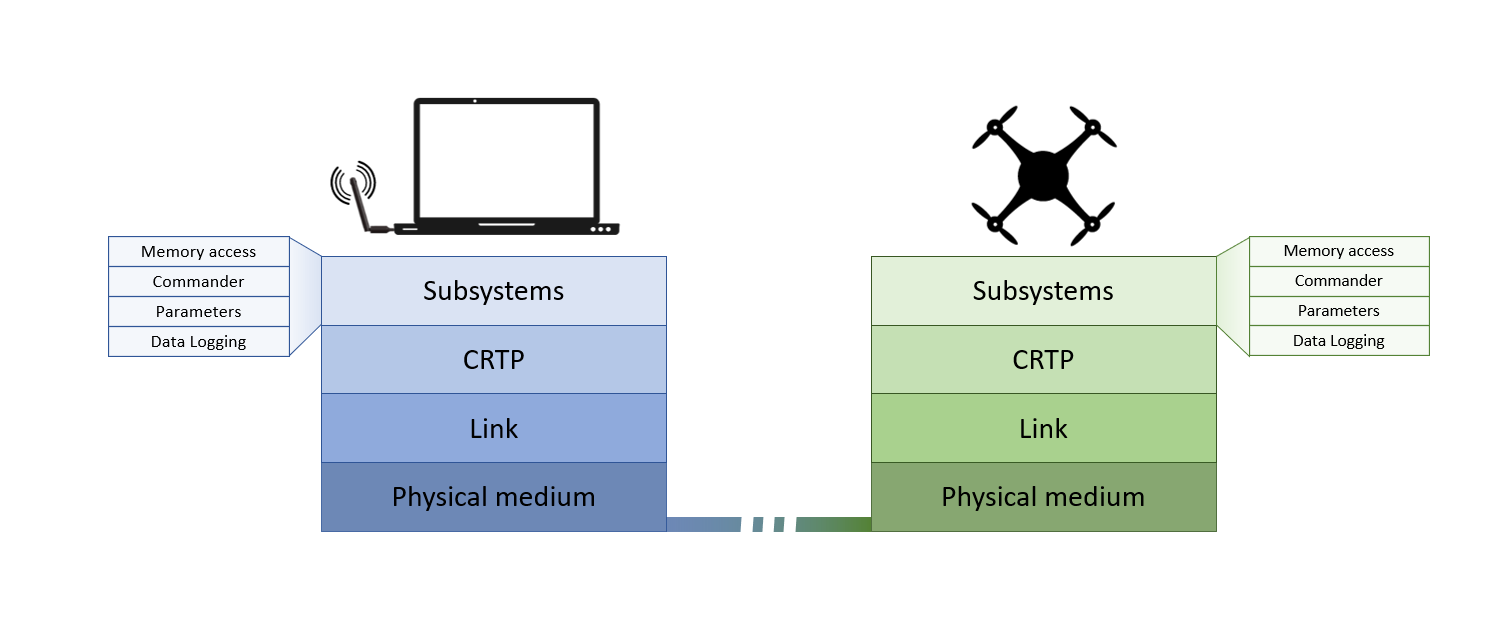
\includegraphics[width=0.5\textwidth]{communication/communication_stack}
    \caption[The Crazyflie communication stack]{The Crayzyflie communication stack is composed of 4 independent layers: Subsystems, CRTP, Link, Physical medium}
    \label{fig:communication_stack}
\end{SCfigure}

In the higher-order layer, we can identify four principal subsystems:
\begin{itemize}
    \item \textbf{Memory access} -- that manages memory operation on the Crazyflie's physical memories, e.g., trajectory uploading.
    \item \textbf{Commander} -- that send/receive control set-points.
    \item \textbf{Parameters} -- that manages read/write operations on configuration parameters of the Crazyflie.
    \item \textbf{Data Logging} -- that handles logs of telemetry data sent periodically from the Crazyflie to the ground station. 
\end{itemize} 

The first two subsystems (memory access and commander) are the simplest, with a straightforward implementation. 
They expose some methods through an API, and when called, they craft a packet, fill it with parameters data, and send it to the link layer.
On the other side, the same subsystem receives the packet, unpacks the data, and executes the desired function.

Conversely, the parameters and data logging subsystems have some peculiarities that make them more complex. 
In particular, the parameters subsystem allows performing read/write operations with acknowledgments of the successful operation.
The data logging subsystem, instead, must support periodical updates of telemetry data.
Moreover, both the two subsystems must handle a variety of variables with different types.

The Communication Framework that we designed and developed is meant to wrap the functionalities of these two complex subsystems and offer the user a more usable and efficient way to handle data logging and parameters.

\section{The Design of the Communication Framework}\label{sec:communication_frameworks_design}
\subsection{The Logging Manager}\label{subsec:logging_manager}
\subsection{The Parameter Manager}\label{subsec:parameter_manager}
